\section{Level-Sets}
{
\setbeamertemplate{background}{}
\setbeamertemplate{navigation symbols}{}
\setbeamercolor{background canvas}{bg={black}}
\color{white}
\begin{frame}[plain]
\fontsize{36pt}{36pt}\selectfont
\center
\begin{center}
Refactored Level Sets
\vskip12pt
\end{center}

\fontsize{12pt}{12pt}\selectfont
Insight Software Consortium\\
Megason Lab, Department of Systems Biology\\
Harvard Medical School
\vskip12pt
\begin{tabular}{cp{.3\textwidth}p{.3\textwidth}p{.3\textwidth}c}
\\
\\
&
\centering{}Arnaud Gelas &
\centering{}Kishore Mosaliganti &
\centering{}Sean Megason & \\
\end{tabular}
\end{frame}
}

\subsection{Introduction}
\centeredlargetext{white}{black}{
Introduction
}

%%%%%%%%%%%%%%%%%%%%%%%%%%%%%%%%%%%%%%%%%%%%%%%%%%%%%%%%%%%%%%%%%%%%%%%%%%%%%%%%
%%%%%%%%%%%%%%%%%%%%%%%%%%%%%%%%%%%%%%%%%%%%%%%%%%%%%%%%%%%%%%%%%%%%%%%%%%%%%%%%
%%%%%%%%%%%%%%%%%%%%%%%%%%%%%%%%%%%%%%%%%%%%%%%%%%%%%%%%%%%%%%%%%%%%%%%%%%%%%%%%

\begin{frame}
\frametitle{What is a level-set function?}

\begin{columns}
\column{0.55\textwidth}
\begin{block}{Definition}
\begin{itemize}
\item Implicit function $\phi : \Omega \rightarrow \mathbb{R}$
\item If $\phi(p) = 0$, $p$ is on the interface $\Gamma$
\item If $\phi(p) < 0$, $p$ is inside
\item Else $p$ is outside
\end{itemize}
\end{block}
\column{0.35\textwidth}
\begin{center}
 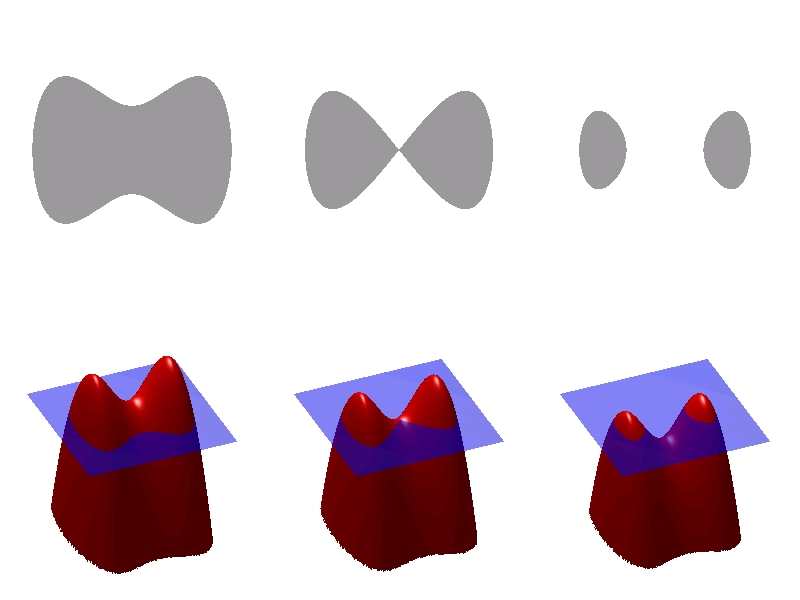
\includegraphics[width=0.9\textwidth]{../Art/Level_set_method.jpg}
\end{center}

\end{columns}

\end{frame}

%%%%%%%%%%%%%%%%%%%%%%%%%%%%%%%%%%%%%%%%%%%%%%%%%%%%%%%%%%%%%%%%%%%%%%%%%%%%%%%%
%%%%%%%%%%%%%%%%%%%%%%%%%%%%%%%%%%%%%%%%%%%%%%%%%%%%%%%%%%%%%%%%%%%%%%%%%%%%%%%%
%%%%%%%%%%%%%%%%%%%%%%%%%%%%%%%%%%%%%%%%%%%%%%%%%%%%%%%%%%%%%%%%%%%%%%%%%%%%%%%%

\begin{frame}
\frametitle{Level-Set Evolution}
\begin{itemize}
  \item Deforms the level-set function
  \begin{itemize}
    \item Driven by given PDE
    \begin{itemize}
      \item<2->Regularized Advection
      \begin{equation*}
      \frac{\partial \phi}{\partial \tau} =
      \alpha \cdot \overrightarrow{A}(p) \bullet \overrightarrow{\nabla} \phi +
      \gamma \cdot \text{div}\left( \frac{\overrightarrow{\nabla}
      \phi}{\|\overrightarrow{\nabla} \phi\|} \right) \cdot
    \|\overrightarrow{\nabla}
      \phi\|
      \end{equation*}
      \only<2>{
      \begin{columns}
        \column{0.3\textwidth}
        \begin{block}{Advection}
        \begin{center}
          $\alpha \cdot \overrightarrow{A}(p) \bullet \overrightarrow{\nabla}
\phi$ \\
        \end{center}
        $\alpha$: coefficient\\
        $A(p)$: Advection field
        \end{block}

        \column{0.3\textwidth}
        \begin{block}{Curvature}
        \begin{center}
          $\gamma \cdot \|\overrightarrow{\nabla} \phi\| \cdot
            \text{div}\ \frac{\overrightarrow{\nabla}
            \phi}{\|\overrightarrow{\nabla} \phi\|}$\\
        \end{center}
          $\gamma$: coefficient
        \end{block}
      \end{columns}
    }

      \item<3->Regularized Propagation
      \begin{equation*}
      \frac{\partial \phi}{\partial \tau} =
      \beta \cdot P(p) \cdot \|\overrightarrow{\nabla} \phi \| +
      \gamma \cdot \text{div}\left( \frac{\overrightarrow{\nabla}
      \phi}{\|\overrightarrow{\nabla} \phi\|} \right) \cdot
    \|\overrightarrow{\nabla}
      \phi\|
      \end{equation*}
      \only<3>{
      \begin{columns}
        \column{0.3\textwidth}
        \begin{block}<3>{Propagation}
          \begin{center}
          $\beta \cdot P(p) \cdot \|\overrightarrow{\nabla} \phi\|$ \\
          \end{center}
          $\beta$: coefficient \\
          $P(p)$: Propagation field
        \end{block}

        \column{0.3\textwidth}
        \begin{block}{Curvature}
          \begin{center}
          $\gamma \cdot \|\overrightarrow{\nabla} \phi\| \cdot
            \text{div}\ \frac{\overrightarrow{\nabla}
            \phi}{\|\overrightarrow{\nabla} \phi\|}$\\
          \end{center}
          $\gamma$: coefficient
        \end{block}
      \end{columns}
      }
      \item<4->Chan and Vese
      \begin{equation*}
      \frac{\partial \phi}{\partial \tau} = \delta_{\epsilon}(\phi)
      \left(
      - \lambda_{in} \left( I - \mu_{in} \right) +
      \lambda_{out} \left( I - \mu_{out} \right)
      \right)
      \end{equation*}
      \only<4>{
      \begin{columns}
        \column{0.4\textwidth}
        \begin{block}{Chan And Vese Internal}
          \begin{center}
          $\delta_{\epsilon}(\phi) \left( \lambda_{in} \left( I - \mu_{in}
\right)\right)$ \\
          \end{center}
          $\lambda_{in}$: coefficient \\
          $\mu_{in}$: Internal Mean
        \end{block}

        \column{0.4\textwidth}
        \begin{block}{Chan And Vese External}
          \begin{center}
          $\delta_{\epsilon}(\phi) \left( \lambda_{out} \left( I - \mu_{out}
\right)\right)$ \\
          \end{center}
          $\lambda_{out}$: coefficient \\
          $\mu_{out}$: External Mean
        \end{block}
      \end{columns}
      }
    \end{itemize}
  \end{itemize}
\end{itemize}
\end{frame}

%%%%%%%%%%%%%%%%%%%%%%%%%%%%%%%%%%%%%%%%%%%%%%%%%%%%%%%%%%%%%%%%%%%%%%%%%%%%%%%%
%%%%%%%%%%%%%%%%%%%%%%%%%%%%%%%%%%%%%%%%%%%%%%%%%%%%%%%%%%%%%%%%%%%%%%%%%%%%%%%%
%%%%%%%%%%%%%%%%%%%%%%%%%%%%%%%%%%%%%%%%%%%%%%%%%%%%%%%%%%%%%%%%%%%%%%%%%%%%%%%%

\begin{frame}
\frametitle{Level-Set Evolution}
\begin{itemize}
  \item Iterative computation
  \item Topological flexibility
\end{itemize}
\end{frame}


%%%%%%%%%%%%%%%%%%%%%%%%%%%%%%%%%%%%%%%%%%%%%%%%%%%%%%%%%%%%%%%%%%%%%%%%%%%%%%%%
%%%%%%%%%%%%%%%%%%%%%%%%%%%%%%%%%%%%%%%%%%%%%%%%%%%%%%%%%%%%%%%%%%%%%%%%%%%%%%%%
%%%%%%%%%%%%%%%%%%%%%%%%%%%%%%%%%%%%%%%%%%%%%%%%%%%%%%%%%%%%%%%%%%%%%%%%%%%%%%%%

\begin{frame}
\frametitle{Level Sets: Challenges in Segmentation?}
\begin{itemize}
  \item PDE Term choice
    \begin{itemize}
      \item Advection terms ?
      \item Propagation terms ?
      \item Region terms ?
      \item Regularization terms ?
    \end{itemize}
  \item<2-> Stopping criterion
    \begin{itemize}
      \item Number of Iterations ?
      \item Variation of interface length / area ?
      \item Variation of shape area / volume ?
    \end{itemize}
  \item<3-> PDE Parameters tuning
\end{itemize}
\end{frame}


%%%%%%%%%%%%%%%%%%%%%%%%%%%%%%%%%%%%%%%%%%%%%%%%%%%%%%%%%%%%%%%%%%%%%%%%%%%%%%%%
%%%%%%%%%%%%%%%%%%%%%%%%%%%%%%%%%%%%%%%%%%%%%%%%%%%%%%%%%%%%%%%%%%%%%%%%%%%%%%%%
%%%%%%%%%%%%%%%%%%%%%%%%%%%%%%%%%%%%%%%%%%%%%%%%%%%%%%%%%%%%%%%%%%%%%%%%%%%%%%%%

\begin{frame}
\frametitle{Level Sets Representation}
\begin{columns}
\column{0.45\textwidth}
\begin{block}{Discrete}
  \begin{itemize}
  \item Dense
  \item<2-> Sparse
  \begin{enumerate}
      \item<3-> Whitaker
      \item<4-> Shi
      \item<5-> Malcolm
    \end{enumerate}
  \end{itemize}
\end{block}

\begin{block}<6->{Parametric}
  \begin{itemize}
    \item<6-> \alert<6>{Easy integration of new representation}
  \end{itemize}
\end{block}

\column{0.45\textwidth}
\only<3>{
\begin{center}
 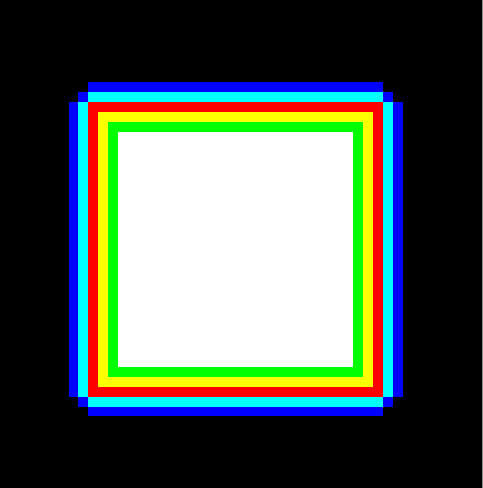
\includegraphics[width=0.8\textwidth]{../Art/WhitakerLayers.png}
 % WhitakerLayers.png: 483x488 pixel, 72dpi, 17.04x17.21 cm, bb=0 0 483 488
\end{center}
}
\only<4>{
\begin{center}
 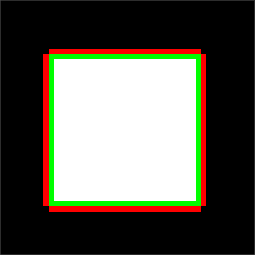
\includegraphics[width=0.8\textwidth]{../Art/ShiLayers.png}
 % WhitakerLayers.png: 483x488 pixel, 72dpi, 17.04x17.21 cm, bb=0 0 483 488
\end{center}
}
\only<5->{
\begin{center}
 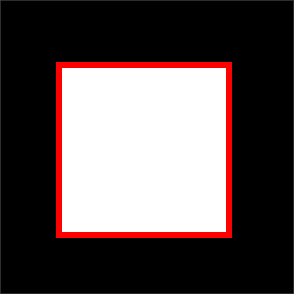
\includegraphics[width=0.8\textwidth]{../Art/MalcolmLayers.png}
 % WhitakerLayers.png: 483x488 pixel, 72dpi, 17.04x17.21 cm, bb=0 0 483 488
\end{center}
}

\end{columns}

\end{frame}

%%%%%%%%%%%%%%%%%%%%%%%%%%%%%%%%%%%%%%%%%%%%%%%%%%%%%%%%%%%%%%%%%%%%%%%%%%%%%%%%
%%%%%%%%%%%%%%%%%%%%%%%%%%%%%%%%%%%%%%%%%%%%%%%%%%%%%%%%%%%%%%%%%%%%%%%%%%%%%%%%
%%%%%%%%%%%%%%%%%%%%%%%%%%%%%%%%%%%%%%%%%%%%%%%%%%%%%%%%%%%%%%%%%%%%%%%%%%%%%%%%

\begin{frame}
\frametitle{Level Sets Equation}

\begin{columns}
  \column{0.47\textwidth}
  \begin{block}{Term}
    \begin{itemize}
      \item Contribution for $\phi$ evolution
      \item Contribution for time step computation
      \item Coefficient
    \end{itemize}
  \alert<2>{Easy to contribute new terms!}
  \end{block}

  \column{0.47\textwidth}
  \begin{block}<3->{TermContainer}
    \begin{itemize}
      \item Represent a given PDEs
      \item Mix of any term
      \item Independent of the representation
    \end{itemize}
  \alert<4>{Easy to contribute new PDEs!}
  \end{block}

\end{columns}

\end{frame}

%%%%%%%%%%%%%%%%%%%%%%%%%%%%%%%%%%%%%%%%%%%%%%%%%%%%%%%%%%%%%%%%%%%%%%%%%%%%%%%%
%%%%%%%%%%%%%%%%%%%%%%%%%%%%%%%%%%%%%%%%%%%%%%%%%%%%%%%%%%%%%%%%%%%%%%%%%%%%%%%%
%%%%%%%%%%%%%%%%%%%%%%%%%%%%%%%%%%%%%%%%%%%%%%%%%%%%%%%%%%%%%%%%%%%%%%%%%%%%%%%%

\begin{frame}
\frametitle{Other Features}
  \begin{itemize}
    \item N Level-Sets function evolving at the same time
    \item Geometrical Constraints
  \end{itemize}
\end{frame}

%%%%%%%%%%%%%%%%%%%%%%%%%%%%%%%%%%%%%%%%%%%%%%%%%%%%%%%%%%%%%%%%%%%%%%%%%%%%%%%%
%%%%%%%%%%%%%%%%%%%%%%%%%%%%%%%%%%%%%%%%%%%%%%%%%%%%%%%%%%%%%%%%%%%%%%%%%%%%%%%%
%%%%%%%%%%%%%%%%%%%%%%%%%%%%%%%%%%%%%%%%%%%%%%%%%%%%%%%%%%%%%%%%%%%%%%%%%%%%%%%%
\subsection{Example}

%%%%%%%%%%%%%%%%%%%%%%%%%%%%%%%%%%%%%%%%%%%%%%%%%%%%%%%%%%%%%%%%%%%%%%%%%%%%%%%%
%%%%%%%%%%%%%%%%%%%%%%%%%%%%%%%%%%%%%%%%%%%%%%%%%%%%%%%%%%%%%%%%%%%%%%%%%%%%%%%%
%%%%%%%%%%%%%%%%%%%%%%%%%%%%%%%%%%%%%%%%%%%%%%%%%%%%%%%%%%%%%%%%%%%%%%%%%%%%%%%%

\begin{frame}[fragile]
  \frametitle{How to run the example?}
  \fontsize{8pt}{8pt}\selectfont
\begin{verbatim}
cd ~/bin/ITKv4-TheNextGeneration-Tutorial/bin/
\end{verbatim}

\begin{verbatim}
./SingleLevelSetWhitaker
    <InputImage>
    <NumberOfIterations>
    <Visualization (0 or 1)>
    <OutputImage>
\end{verbatim}

\begin{verbatim}
./SingleLevelSetWhitaker
    ~/data/cells.png
    800
    1
    cells_segmented.mha
\end{verbatim}
\end{frame}
\centeredlargetext{white}{black}{
Example\\
Code Walk-Through
}

\begin{frame}
  \frametitle{Create a level-set function from binary mask}
  \lstlistingwithnumber{53}{53}{SingleLevelSetWhitaker.cxx}
  \lstlistingwithnumber{96}{106}{SingleLevelSetWhitaker.cxx}
  \lstlistingwithnumber{110}{112}{SingleLevelSetWhitaker.cxx}
\end{frame}

%%%%%%%%%%%%%%%%%%%%%%%%%%%%%%%%%%%%%%%%%%%%%%%%%%%%%%%%%%%%%%%%%%%%%%%%%%%%%%%%
%%%%%%%%%%%%%%%%%%%%%%%%%%%%%%%%%%%%%%%%%%%%%%%%%%%%%%%%%%%%%%%%%%%%%%%%%%%%%%%%
%%%%%%%%%%%%%%%%%%%%%%%%%%%%%%%%%%%%%%%%%%%%%%%%%%%%%%%%%%%%%%%%%%%%%%%%%%%%%%%%

\begin{frame}
  \frametitle{Create a domain for the level-set function}
  \lstlistingwithnumber{118}{122}{SingleLevelSetWhitaker.cxx}
  \lstlistingwithnumber{126}{137}{SingleLevelSetWhitaker.cxx}
\end{frame}

%%%%%%%%%%%%%%%%%%%%%%%%%%%%%%%%%%%%%%%%%%%%%%%%%%%%%%%%%%%%%%%%%%%%%%%%%%%%%%%%
%%%%%%%%%%%%%%%%%%%%%%%%%%%%%%%%%%%%%%%%%%%%%%%%%%%%%%%%%%%%%%%%%%%%%%%%%%%%%%%%
%%%%%%%%%%%%%%%%%%%%%%%%%%%%%%%%%%%%%%%%%%%%%%%%%%%%%%%%%%%%%%%%%%%%%%%%%%%%%%%%

\begin{frame}
  \frametitle{Setting up the level-set container}
  \lstlistingwithnumber{141}{146}{SingleLevelSetWhitaker.cxx}
  \lstlistingwithnumber{149}{156}{SingleLevelSetWhitaker.cxx}
\end{frame}

%%%%%%%%%%%%%%%%%%%%%%%%%%%%%%%%%%%%%%%%%%%%%%%%%%%%%%%%%%%%%%%%%%%%%%%%%%%%%%%%
%%%%%%%%%%%%%%%%%%%%%%%%%%%%%%%%%%%%%%%%%%%%%%%%%%%%%%%%%%%%%%%%%%%%%%%%%%%%%%%%
%%%%%%%%%%%%%%%%%%%%%%%%%%%%%%%%%%%%%%%%%%%%%%%%%%%%%%%%%%%%%%%%%%%%%%%%%%%%%%%%

\begin{frame}
  \frametitle{Creating PDE Terms}
  \begin{itemize}
    \item Chan and Vese internal term
    \lstlistingwithnumber{163}{170}{SingleLevelSetWhitaker.cxx}
    \item Chan and Vese external term
    \lstlistingwithnumber{174}{181}{SingleLevelSetWhitaker.cxx}
  \end{itemize}
\end{frame}

%%%%%%%%%%%%%%%%%%%%%%%%%%%%%%%%%%%%%%%%%%%%%%%%%%%%%%%%%%%%%%%%%%%%%%%%%%%%%%%%
%%%%%%%%%%%%%%%%%%%%%%%%%%%%%%%%%%%%%%%%%%%%%%%%%%%%%%%%%%%%%%%%%%%%%%%%%%%%%%%%
%%%%%%%%%%%%%%%%%%%%%%%%%%%%%%%%%%%%%%%%%%%%%%%%%%%%%%%%%%%%%%%%%%%%%%%%%%%%%%%%

\begin{frame}
  \frametitle{Setting up PDE}
  \lstlistingwithnumber{187}{195}{SingleLevelSetWhitaker.cxx}
  \lstlistingwithnumber{199}{202}{SingleLevelSetWhitaker.cxx}
\end{frame}

%%%%%%%%%%%%%%%%%%%%%%%%%%%%%%%%%%%%%%%%%%%%%%%%%%%%%%%%%%%%%%%%%%%%%%%%%%%%%%%%
%%%%%%%%%%%%%%%%%%%%%%%%%%%%%%%%%%%%%%%%%%%%%%%%%%%%%%%%%%%%%%%%%%%%%%%%%%%%%%%%
%%%%%%%%%%%%%%%%%%%%%%%%%%%%%%%%%%%%%%%%%%%%%%%%%%%%%%%%%%%%%%%%%%%%%%%%%%%%%%%%

\begin{frame}
  \frametitle{Stopping criterion}
  \lstlistingwithnumber{204}{208}{SingleLevelSetWhitaker.cxx}
\end{frame}

%%%%%%%%%%%%%%%%%%%%%%%%%%%%%%%%%%%%%%%%%%%%%%%%%%%%%%%%%%%%%%%%%%%%%%%%%%%%%%%%
%%%%%%%%%%%%%%%%%%%%%%%%%%%%%%%%%%%%%%%%%%%%%%%%%%%%%%%%%%%%%%%%%%%%%%%%%%%%%%%%
%%%%%%%%%%%%%%%%%%%%%%%%%%%%%%%%%%%%%%%%%%%%%%%%%%%%%%%%%%%%%%%%%%%%%%%%%%%%%%%%

\begin{frame}
  \frametitle{Starts the evolution}
  \begin{itemize}
    \item Set a stopping criterion
    \lstlistingwithnumber{223}{223}{SingleLevelSetWhitaker.cxx}
    \item Evolve
    \lstlistingwithnumber{225}{236}{SingleLevelSetWhitaker.cxx}
  \end{itemize}
\end{frame}

%%%%%%%%%%%%%%%%%%%%%%%%%%%%%%%%%%%%%%%%%%%%%%%%%%%%%%%%%%%%%%%%%%%%%%%%%%%%%%%%
%%%%%%%%%%%%%%%%%%%%%%%%%%%%%%%%%%%%%%%%%%%%%%%%%%%%%%%%%%%%%%%%%%%%%%%%%%%%%%%%
%%%%%%%%%%%%%%%%%%%%%%%%%%%%%%%%%%%%%%%%%%%%%%%%%%%%%%%%%%%%%%%%%%%%%%%%%%%%%%%%

\subsection{Exercise}
\centeredlargetext{white}{black}{
Exercise: Add a curvature term to LevelSetExercise1.cxx
}

%%%%%%%%%%%%%%%%%%%%%%%%%%%%%%%%%%%%%%%%%%%%%%%%%%%%%%%%%%%%%%%%%%%%%%%%%%%%%%%%
%%%%%%%%%%%%%%%%%%%%%%%%%%%%%%%%%%%%%%%%%%%%%%%%%%%%%%%%%%%%%%%%%%%%%%%%%%%%%%%%
%%%%%%%%%%%%%%%%%%%%%%%%%%%%%%%%%%%%%%%%%%%%%%%%%%%%%%%%%%%%%%%%%%%%%%%%%%%%%%%%

% \begin{frame}
% \frametitle{Multi Level Sets}
% \begin{itemize}
%   \item N Level Sets function evolving at the same time
%   \item Geometrical Constraints
% \end{itemize}
% \end{frame}
%
% \end{colum}


%\begin{frame}
%\frametitle{Wrap-up}
%\begin{itemize}
  %\item Send us feedback (good or bad)
  %\begin{itemize}
    %\item \url{arnaudgelas@gmail.com}
    %\item \url{kishore_mosaliganti@hms.harvard.edu}
    %\item \url{sean_megason@hms.harvard.edu}
    %\item \url{insight-users@public.kitware.com}
  %\end{itemize}
%\end{itemize}
%\end{frame}
